\section{Abbildungen und Funktionen}
\subsection{Grundbegriffe}
Eine Abbildung $f: A \rightarrow B$ heißt Funktion von A nach B, wenn jedem $a \in A$ genau ein $b \in B$ zugeordnet wird. $b = f(a)$ heißt Funktionswert an der Stelle $a$. Der Definitionsbereich $\mathbb{D}$ sind die Werte,  die in die Funktion als $a$ eingegeben werden können. Der Wertebereich $\mathbb{W}$ sind die Werte, die aus der Funktion resultieren. Die Bereiche können als übliche Mengen mit Eigenschaft niedergeschrieben werden z.B. :
\begin{align*}
\mathbb{D}(f(x)) &= \{ x \in \mathbb{R} \enspace | \enspace x \}\\
\mathbb{W}(f(x)) &= \{ y \in \mathbb{R} \enspace | \enspace y \}
\end{align*}
\subsection{Gerade und ungerade Funktion}
\begin{align*}
f(-x) &= f(x) &\text{Gerade Funktion}\\ 
f(-x) &= -f(x) &\text{Ungerade Funktion}
\end{align*}
\subsection{Periodische Funktionen}
\begin{align*}
f(x+\lambda ) = f(x)
\end{align*}
Kleinstes $\lambda > 0$ ist die \underline{primitive Periode}.
\subsubsection{Beschränktheit}
Es sei $f: A \rightarrow B$. $M \subset A$ beschränkt an $K$.\\
Beispiel: $f(x) = \sin{x}$
$$| \sin{x} | \leq 1 \quad \forall x \in \mathbb{R}$$
Kleinste obere Schranke einer Funktion heißt \underline{Supremum}.
\begin{align*}
f(x) &= \sin{x}\\
\sup{f} &= 1
\end{align*}
Größte untere Schranke heißt \underline{Infimum}.
\begin{align*}
\inf{f} &= -1
\end{align*}
\subsubsection{Monotonieverhalten}
Eine Funktion $f: A \rightarrow B$ heißt im Intervall $I \subset A$ monoton wachsend bzw. streng monoton wachsend, wenn $\forall x_1,x_2 \in I$ mit $x_1 > x_2$ die Ungleichung 
$$f(x_1) \geq f(x_2) \quad \text{bzw.} \quad f(x_1) > f(x_2)$$
gilt. Entsprechend heißt sie monoton fallend bzw. streng monoton fallend, wenn $\forall x_1,x_2 \in I$ mit $x_1 > x_2$ die Ungleichung
$$f(x_1) \leq f(x_2) \quad \text{bzw.} \quad f(x_1) < f(x_2)$$
\subsection{Elementare Funktionen}
\subsubsection{Polynome}
Ein Polynom ist definiert durch:
$$f(x) = a_0 + a_1 x + \cdots + a_n x^n = \sum_{k=0}^n a_k x^k$$
Addition/Subtraktion:
$$\sum_{k=0}^n a_k x^k \pm \sum_{k=0}^n b_k x^k = \sum_{k=0}^n (a_k \pm b_k) x^k$$
Multiplikation:
$$\sum_{k=0}^n a_k x^k \cdot \sum_{k=0}^n b_k x^k = \sum_{k=0}^n a_k x^k \cdot \sum_{l=0}^n b_l x^l = \sum_{k=0}^n \sum_{l=0}^n a_k b_l x^{k+l}$$
\subsubsection{Lineare Funktion}
Die Hauptform der linearen Funktion lautet $f(x) = a_0 + a_1 x$. $a_0$ und $a_1$ können mit zwei Wertepaaren von $f(x)$ bestimmt werden:
\begin{align*}
a_1 &= \frac{y_2 - y_1}{x_2 - x_1}\\
a_0 &= y_1 - \frac{y_2 - y_1}{x_2 - x_1}x_1 = \frac{y_1 x_2 - y_2 x_1}{x_2 - x_1}
\end{align*}
Die Zweipunktform der linearen Funktion lautet $\frac{y - y_1}{x - x_1} = \frac{y_2 - y_1}{x_2 - x_1}$.\\
Die Achsenabschnittsform lautet $\frac{x}{a} + \frac{y}{b} = 1$. Mit $f(0) = b$ und $f(a)=0$.
\subsubsection{Quadratische Funktion}
Die Hauptform der quadratischen Funktion lautet $f(x) = a_0 + a_1 x + a_2 x^2$.\\
Die Nullstellen der quadratischen Funktion lassen sich über die p,q-Formel bestimmen. Diese leitet sich aus der Hauptform her:
\begin{align*}
a_2 x^2 + a_1 x + a_0 &= 0 &:a_2\\
x^2 + p x + q &= 0 &\text{mit $p = \frac{a_1}{a_2}, q = \frac{a_0}{a_2}$}\\
\Rightarrow x_{1/2} &= - \frac{p}{2} \pm \sqrt{(\frac{p}{2})^2 - q} &\text{p,q-Formel}
\end{align*}
Die Nullstellen lassen sich ebenfalls mithilfe der Mitternachtsformel bestimmen:
\begin{align*}
x_{1/2} &= \frac{-b \pm \sqrt{b^2 - 4ac}}{2a}\\
\text{Diskriminante} \quad D &= b^2 - 4ac\\
\end{align*}
Dabei gelten für die Diskriminante $D$ folgende Eigenschaften und Folgen für die Funktion:
\begin{tabular}{c l}
$D>0$ & reelle Lösung $x_1 | x_2$ \\
$D=0$ & eine doppelte reelle Lösung\\
$D<0$ & zwei Lösungen in $\mathbb{C}$ die konjugiert-komplex zueinander sind\\
\end{tabular}
\paragraph{Wurzelsatz von Vi\"{e}ta} ist für $\mathbb{C}$ als auch $\mathbb{R}$ gültig und lautet:
\begin{align*}
p &= -(x_1 + x_2)\\
q &= x_1 \cdot x_2
\end{align*}
\paragraph{Das Horner-Schema} erlaubt es in wenigen Rechenschritten Nullstellen als auch Funktionswerte zu berechnen. Diese Methode erweist sich als einfach für Computerprogramme zu implementieren. Außerdem erlaubt es die Berechnung von Funktionswerten ohne Taschenrechner\footnote{ Als Beispiel:
$11 + 7x - 5x^2 -4x^3 + 2x^4 \;=\; 11 + x \cdot\left(7 + x \cdot(-5 + x \cdot(-4 + x \cdot 2))\right)$}\\
Beispiel: $f(x) = 5x^6 - 2x^5 + 2x^3 + x^2 - 6x +1$. Zur Berechnung vom Funktionswert $f(2)$ sieht das Horner-Schema wie folgt aus:\\

\begin{figure}[!ht]
\caption{Horner-Schema für $f(x)$}
\centering
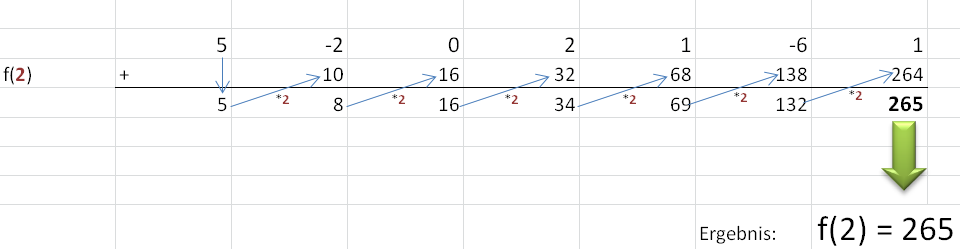
\includegraphics[scale=0.55]{img/img1}
\end{figure}

